\section{Matriz de Confusión}

La matriz de confusion es una técnica que facilita el análisis del rendimiento de un algoritmo de clasificación. Frecuentemente, el rendimiento de un clasificador es solo analizado en términos de la \textit{precision} (verdaderos positivos, verdaderos negativos y falsos positivos). Sin embargo, este no refleja completamente el verdadero rendimiento del clasificador. Así, comunmente es considerado el \textit{recall} para solucionar parcialmente este problema. El \textit{recall} toma en cuenta los falsos negativos (repuestas predichas como falsas cuando en realidad son verdaderas). Adicionalmente, para evaluar el rendimiento final de un clasificador en forma completa se usa el \textit{f1-score}. El f1-score toma en consideración tanto la \textit{precision} y el \textit{recall}, obtiendo una penalización del rendimiento del clasificador cada vez que este se equivoque \cite{30Mconfusion}.
Así, la matriz de confusión cumple un papel importante en el calculo de \textit{precision}, \textit{recall} y \textit{f1-score}. En la Tabla \ref{tab:estruc_confusion_matrix} se puede observar la estructura general de una  matriz de confusión. así mismo en las ecuaciones \ref{eq:Aprecision} y \ref{eq:Arecall}  se muestra el uso de los elementos la matriz de confusión para calcular las métricas de \textit{precision} y \textit{recall} respectivamente. Finalmente, la ecuación \ref{eq:Af1score} muestra el cálculo de \textit{f1-score}. 


\begin{table}[!htb]
  
  \noindent
  \renewcommand\arraystretch{1.5}
  \setlength\tabcolsep{0pt}
  \begin{center}
  \begin{tabular}{c >{\bfseries}r @{\hspace{0.7em}}c @{\hspace{0.4em}}c @{\hspace{0.7em}}l}
    \multirow{10}{*}{\rotatebox{90}{\parbox{1.1cm}  { \bfseries\centering  Valores \\ predichos}}} & 
      & \multicolumn{2}{c}{\bfseries Valores referenciales} & \\
    & & \bfseries Positivos & \bfseries Negativos \\
    & {Positivos} & \MyBox{True}{Positive (TP)} & \MyBox{False}{Negative (FN)} \\[2.4em]
    & Negativos & \MyBox{False}{Positive (FP)} & \MyBox{True}{Negative (TN)} \\
  
  \end{tabular}
  \end{center}
    \caption{Estructura general de la matriz de confusión}
        \label{tab:estruc_confusion_matrix}
\end{table}

\begin{equation}\label{eq:Aprecision}
precision = \frac{ TP}{TP+FP}
\end{equation}

\begin{equation}\label{eq:Arecall}
recall = \frac{ TP}{TP+FN}
\end{equation}

\begin{equation}\label{eq:Af1score}
f1-score = \frac{2 \cdot precision\cdot recall}{precision+ recall}
\end{equation}



\section{Machine Learning}

El \textit{machine learnin}g es un area de la la inteligencia artificial que alberga algoritmos de aprendizaje. La definición: “Se dice que un programa de computadora aprende de la experiencia E con respecto a alguna clase de tareas T y la medida de rendimiento P, si su desempeño de tareas en T, medido por P, mejora con la experiencia E.” realizada en \cite{mitchell1997machine} nos explica que significa aprender para una máquina.
 
\section{Aplicaciones de Machine Learning}

Los algoritmos de \textit{machine learning} 
pueden ser usados para una infinidad de aplicaciones que solucionen problemas del mundo real. La amplia gama de aplicaciones en los que pueden ser utilizados los algoritmos de \textit{machine learning} van desde motores de búsqueda, diagnósticos médicos, reconocimiento del habla y del lenguaje, robótica, etc.
Se mencionan algunas de las aplicaciones con mayor tendencia que tienen como elemento principal el uso de algoritmos de \textit{machine learning} \cite{31MLApplications}:


 


\begin{itemize}
\item Detección de rostro.
\item Reconocimiento facial, de voz o de objetos.
\item Motores de Busqueda.
\item Anti-spam.
\item Anti-virus.
\item Genética.
\item Predicción y pronósticos del clima.
\item Comprensión de textos.
\item Vehículos autónomos y robots.
\item Análisis de imágenes de alta calidad.
\item Análisis de datos económicos.
\item Análisis de comportamiento de consumo y productividad.

\end{itemize}


\section{Early Stopping}

%https://deeplearning4j.org/earlystopping

%http://page.mi.fu-berlin.de/prechelt/Biblio/stop_tricks1997.pdf

%https://arxiv.org/pdf/1703.09580.pdf


Cuando se entrena una red neuronal se tiene que definir a priori cuantas iteraciones se harán sobre el conjunto de datos de entrenamiento. 
Depende fuertemente del número de épocas escogido si se obtendrá un buen ajuste a los datos o por el contrario podra ocurrir sobreajuste en los datos de entrenamiento. 

El método de \textit{early stopping}  ayuda a resolver el problema de escoger el número de épocas en el que logra un buen ajuste a los datos de entrenamiento \cite{32Stopping}, \cite{prechelt1998early}.

Los pasos a seguir para la aplicación del método de early stopping son los siguientes:

\begin{itemize}
 \item Dividir la base de datos en 2 partes: base de datos de entrenamiento y base de datos de validación.
 
 \item Para cada N épocas debemos hacer lo siguiente:
   \begin{itemize}
    \item Evaluar el error del modelo en el conjunto de validación.
    \item Parar el entrenamiento si el error de validación es mayor respecto al anterior error de validación.
    \item Finalmente, se selecciona el modelo creado antes del aumento del error de validación.
   \end{itemize}
\end{itemize}

En la Figura \ref{fig:early_stopping} se puede observar la relación época y rendimiento en el conjunto de entrenamiento y el conjunto de validación. Así, como el punto óptimo en el que se alcanza el mejor rendimiento en el conjunto de validación.


\begin{figure}[!htb]
    \centering
    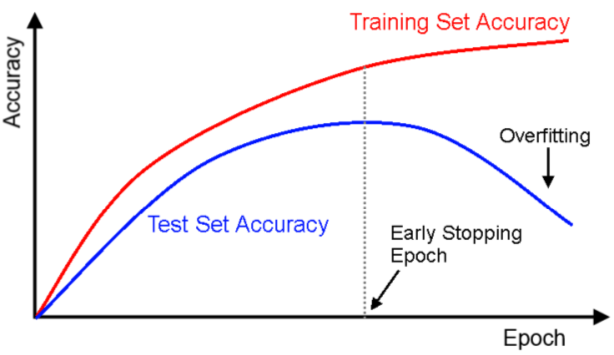
\includegraphics[width=100mm]{Imagenes/early_stopping.png}
    \caption{Representación gráfica de Early Stopping \\ \textit{Fuente: deeplearning4j \cite{32Stopping}}}
    \label{fig:early_stopping}
\end{figure}


